% DO NOT COMPILE THIS FILE DIRECTLY!
% This is included by the other .tex files.

\begin{frame}[t,plain]
    \titlepage
\end{frame}

\begin{frame}[t]{Idea in a nutshell}
\begin{itemize}
\item Capture the public DNS answer packet 
\item at the recursor (not the authoriative NS)
\item delete source IP, destination IP ($\implies$ privacy)
\item timestamp the public DNS record and finally
\item Store it in a DB
\item Provide a Query-Interface
\item Invented by Florian Weimer 2005 (presentation at FIRST.org conference)
\end{itemize}
\end{frame}


\begin{frame}[t]{pre-recursor passive DNS: store-everything-that-you-can approach (potential privacy problem)}
\begin{centering}
  \vbox{}\vfill
  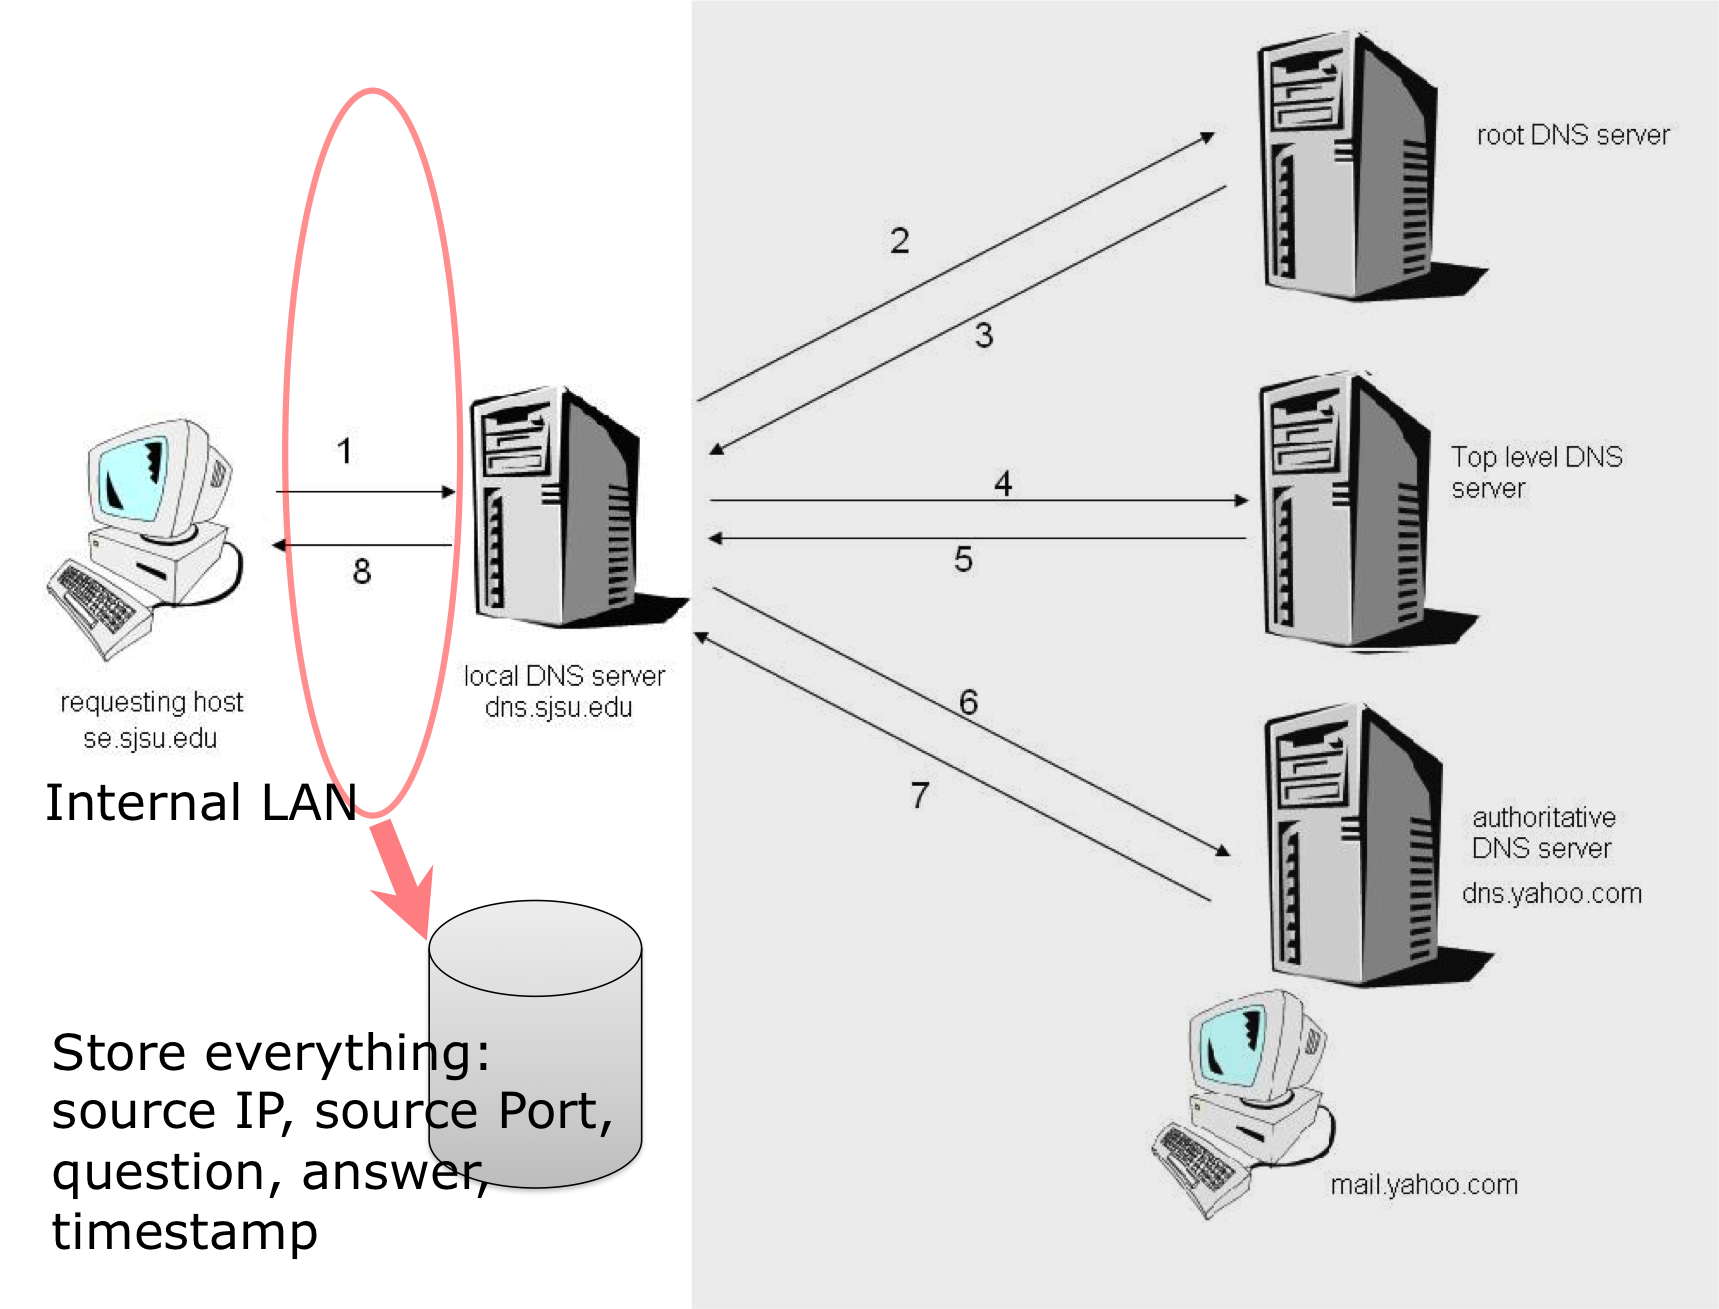
\includegraphics[scale=0.3]{pre-recursor.png}
  \vfill
\end{centering}
\end{frame}

\begin{frame}[t]{post-recursor passive DNS: store only what you need}
\begin{itemize}
\item the original idea. Privacy++. Mix input of different sensors.
\end{itemize}
\begin{centering}
  \vbox{}\vfill
  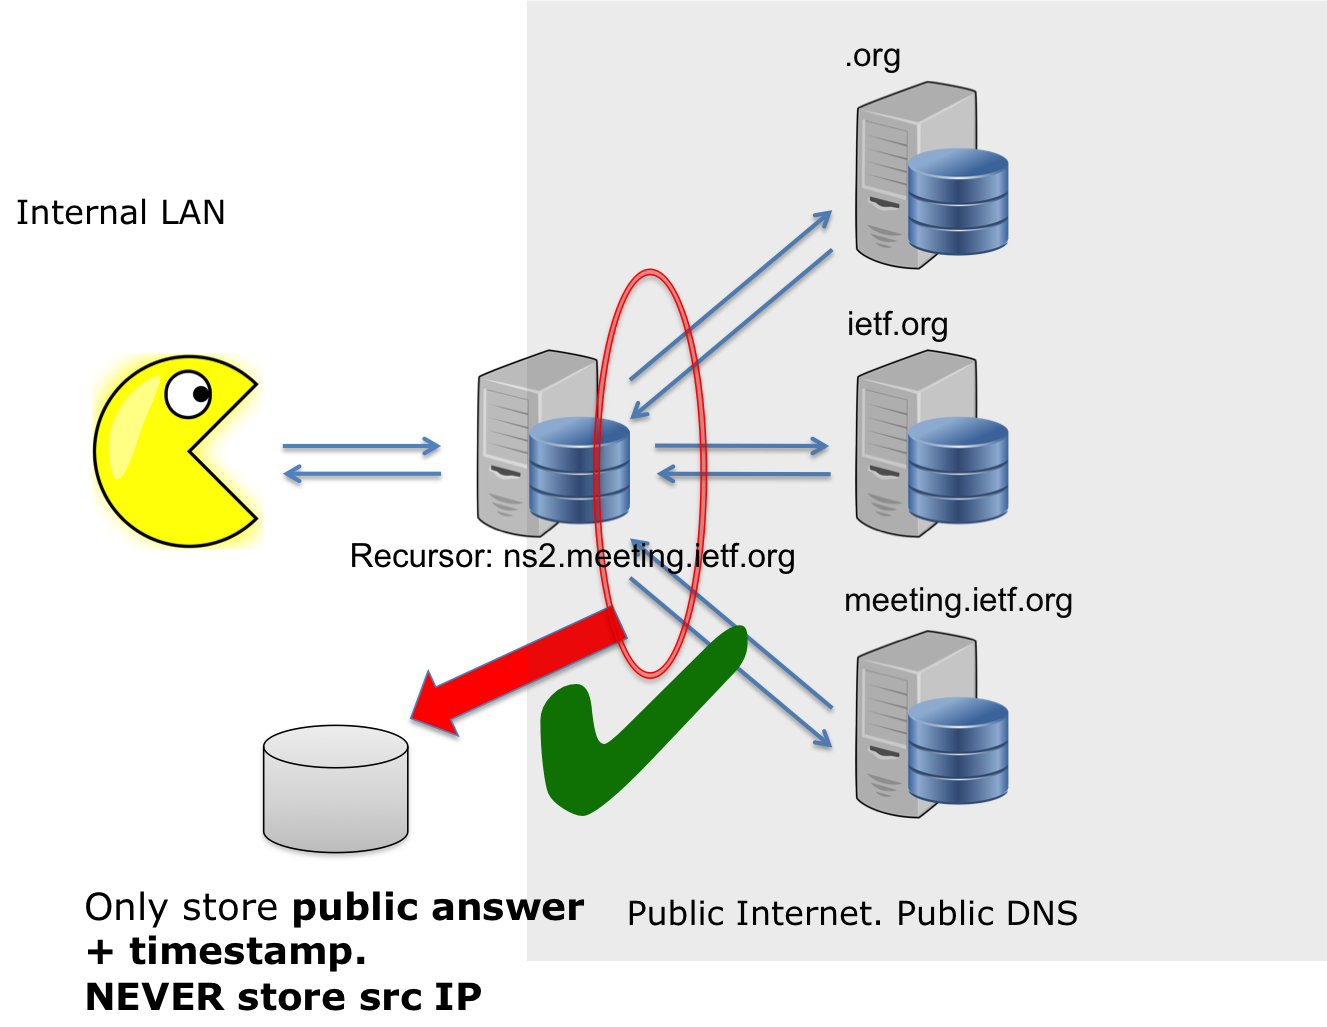
\includegraphics[scale=0.3]{post-recursor.png}
  \vfill
\end{centering}
\end{frame}

\begin{frame}[t]{Why pDNS? Answers which questions?}
\begin{itemize}
\item For example:
\item Historic data: ,,What was the A record for a certain FQDN last year?''
\item Inverse Lookups: ,,Which domains have A records that are in a given address range?''
\item Egypt goes offline: ,,Which domains are offline because all their nameservers are in egyptian IP space?''
\item Generic reseach on bulk DNS data: T. Frosch, T. Holz: ,,Predentifier: Detecting Botnet C\&C Domains From Passive DNS Data''
\item The first time, we can get a sampled subset of \emph{the DNS} per se. I.e.: what is actually out there?
\end{itemize}
\end{frame}

\begin{frame}[t]{Motivation for the I-D}
\begin{itemize}
\item Nowadays Passive DNS servers are created\footnote{To our knowledge, there are more than 15 software implementations} and used worldwide
\item DNS data is very \emph{localized}. It makes sense to have multiple, local DBs (different legal environments, access rights, restrictions to data,...)
\item ... but that means we need a way to \emph{query multiple DBs}.
\item In 2011, we started to work on a \emph{common output format} for Passive DNS systems at the FIRST annual conference
\item After discussions with many authors of passive DNS, version 02 of the internet-draft is published
\end{itemize}
\end{frame}


\begin{frame}[t]{Main objectives of the internet-draft}
\begin{itemize}
\item Consistent naming of fields across Passive DNS software based on the most common Passive DNS implementations
\item Minimal set of fields to be supported
\item Minimal set of optional fields to be supported
\item Way to add "additional" fields via a simple registry mechanism (IANA-like)
\item Simple and easily parsable format
\item A gentle reminder regarding privacy aspects of Passive DNS
\end{itemize}
\end{frame}

\begin{frame}[t,fragile]{Sample output www.terena.org}
\lstdefinelanguage{JavaScript}{
  keywords={typeof, new, true, false, catch, function, return, null, catch, switch, var, if, in, while, do, else, case, break},
  keywordstyle=\color{blue}\bfseries,
  ndkeywords={class, export, boolean, throw, implements, import, this},
  ndkeywordstyle=\color{darkgray}\bfseries,
  identifierstyle=\color{black},
  sensitive=false,
  comment=[l]{//},
  morecomment=[s]{/*}{*/},
  commentstyle=\color{purple}\ttfamily,
  stringstyle=\color{red}\ttfamily,
  morestring=[b]',
  morestring=[b]"
}

\lstset{
   language=JavaScript,
   backgroundcolor=\color{lightgray},
   extendedchars=true,
   basicstyle=\footnotesize\ttfamily,
   showstringspaces=false,
   showspaces=false,
   numbers=left,
   numberstyle=\footnotesize,
   numbersep=9pt,
   tabsize=2,
   breaklines=true,
   showtabs=false,
   captionpos=b
}
\lstset{breaklines=true, language=JavaScript}
\begin{lstlisting}
{"count": 868, "time_first": 1298398002, "rrtype": "A", "rrname": "www.terena.org", "rdata": "192.87.30.6", "time_last": 1383124252}
{"count": 89, "time_first": 1383729690, "rrtype": "CNAME", "rrname": "www.terena.org", "rdata": "godzilla.terena.org", "time_last": 1391517643}
{"count": 110, "time_first": 1298398002, "rrtype": "AAAA", "rrname": "www.terena.org", "rdata": "2001:610:148:dead::6", "time_last": 136670845}
\end{lstlisting}
\end{frame}


\begin{frame}[t]{Mandatory fields}
\begin{itemize}
\item \textbf{rrname} : name of the queried resource records
\begin{itemize}
\item JSON String
\end{itemize}
\item \textbf{rrtype} : resource record type
\begin{itemize}
\item JSON String (interpreted type of resource type if known)
\end{itemize}
\item \textbf{rdata} : resource records of the query(ied) resource(s)
\begin{itemize}
\item JSON String or an array of string if more than one unique triple
\end{itemize}
\item \textbf{time\_first} : first time that the resource record triple (rrname, rrtype, rdata) was seen
\item \textbf{time\_last} : last time that the resource record triple (rrname, rrtype, rdata) was seen
\begin{itemize}
\item JSON Number (epoch value) UTC TZ
\end{itemize}
\end{itemize}
\end{frame}

\begin{frame}[t]{Optional fields}
\begin{itemize}
\item \textbf{count} : how many authoritative DNS answers were received by the Passive DNS collector
\begin{itemize}
\item JSON Number
\end{itemize}
\item \textbf{bailiwick} : closest enclosing zone delegated to a nameserver served in the zone of the resource records
\begin{itemize}
\item JSON String
\end{itemize}

\end{itemize}
\end{frame}

\begin{frame}[t]{Additionals fields}
\begin{itemize}
\item \textbf{sensor\_id} : Passive DNS sensor information
\begin{itemize}
\item JSON String
\end{itemize}
\item \textbf{zone\_time\_first} : specific first/last time seen when imported from a master file
\item \textbf{zone\_time\_last}
\begin{itemize}
\item JSON Number
\end{itemize}
\item Additional fields can be requested via \url{https://github.com/adulau/pdns-qof/wiki/Additional-Fields}
\end{itemize}
\end{frame}


\begin{frame}[t]{Future works}
\begin{itemize}
\item IETF 89 London to review the internet-draft with the dnsop WG
\item Incorporate feedback from dnsop WG
\item Incorporate all the comments and feedback from recently discovered Passive DNS (servers/clients) developers
\item Expand the sample implementations to help developers to support the format
\item An internet-draft for the query interface to Passive DNS systems is under preparation
\end{itemize}
\end{frame}

\begin{frame}[t]{Question}
\begin{center}
\begin{itemize}
\item Is this relevant for DNSOP? WG item?
\end{itemize}
\end{center}
\end{frame}

\begin{frame}[t]{Contact}
\begin{itemize}
\item \url{https://datatracker.ietf.org/doc/draft-dulaunoy-kaplan-passive-dns-cof/}
\item Don't hesitate to contact us. Feedback and updates are welcomed:
\item alexandre.dulaunoy@circl.lu - CIRCL
\item kaplan@cert.at - CERT.at
\item paul@redbarn.org - Farsight Security, Inc
\item henry@stern.ca - Farsight Security, Inc.
\end{itemize}
\end{frame}



